\documentclass[11pt]{article}
\usepackage[margin=1in]{geometry}
\usepackage{amsmath,amssymb}
\usepackage{graphicx}
\usepackage{subcaption}
\usepackage{xcolor}

\title{A 2D Gaussian--Mixture Task:\\ Eight Gaussians on a Circle (and its Ellipse Misspecification)}
\author{tabpfn-misspecification}
\date{\today}

\begin{document}
\maketitle

\section{Model}

We use the 2D instance (\texttt{gaussian\_mixture\_2d}) of the
\texttt{GaussianMixtureHD} task, so the parameter $\theta$ and the data $x$ both
live in $\mathbb{R}^{2}$ ($D=2$). The well-specified generative model is a
\emph{Gaussian prior with a Gaussian-mixture likelihood}, which is conjugate and
therefore yields a closed-form posterior.

\paragraph{Prior.}
\begin{equation}
  \theta \sim \mathcal{N}\!\left(0,\ \sigma_p^2 I_D\right), \qquad \sigma_p = 5 .
\end{equation}
This is a single broad isotropic Gaussian --- there is no mixture in the prior.

\paragraph{Anchors (the ``circle'').}
We fix $K=8$ anchor points evenly spaced on a circle of radius $\rho = 8$:
\begin{equation}
  c_k = \big(\rho\cos\varphi_k,\ \rho\sin\varphi_k\big), \qquad
  \varphi_k = \frac{2\pi k}{K}, \qquad k = 0,\dots,K-1 .
\end{equation}

\paragraph{Likelihood / data-generating process.}
Draw a discrete component $z$, shift $\theta$ by the corresponding anchor, and add
isotropic Gaussian noise:
\begin{equation}
  z \sim \mathrm{Uniform}\{0,\dots,K-1\}, \qquad
  x \mid \theta, z = \theta + c_z + \varepsilon, \qquad
  \varepsilon \sim \mathcal{N}\!\left(0,\ \sigma^2 I_D\right),\ \ \sigma = 0.5 .
\end{equation}
Marginalizing over the component $z$ gives the mixture likelihood
\begin{equation}
  p(x \mid \theta)
  = \frac{1}{K}\sum_{k=0}^{K-1}
      \mathcal{N}\!\left(x;\ \theta + c_k,\ \sigma^2 I_D\right) .
  \label{eq:lik}
\end{equation}
So a data point is the parameter $\theta$ teleported to one of the eight ring
positions, plus a little noise.

\section{Closed-form posterior}

Each term of \eqref{eq:lik} is Gaussian in $\theta$ and the prior is Gaussian, so by
conjugacy (applied per component) the posterior is again a $K$-component Gaussian
mixture:
\begin{equation}
  p(\theta \mid x) = \sum_{k=0}^{K-1} w_k\,
      \mathcal{N}\!\left(\theta;\ \mu_k,\ \tau^2 I_D\right),
\end{equation}
with shared (shrunk) variance, per-component means, and weights
\begin{equation}
  \tau^2 = \frac{\sigma_p^2\,\sigma^2}{\sigma_p^2 + \sigma^2}, \qquad
  \mu_k = \frac{\tau^2}{\sigma^2}\,(x - c_k), \qquad
  w_k \propto \exp\!\left(-\frac{\lVert x - c_k\rVert^2}{2(\sigma_p^2 + \sigma^2)}\right).
  \label{eq:post}
\end{equation}

The reference observation is set to the symmetric point $x_{\mathrm{obs}} = 0$. Then
every $\lVert c_k\rVert = \rho$ is equal, so all weights are equal, $w_k = 1/K$, and the
means reduce to
\begin{equation}
  \mu_k = -\frac{\tau^2}{\sigma^2}\,c_k ,
\end{equation}
i.e.\ \emph{eight equal-weight, isotropic blobs} (standard deviation $\tau$) sitting on a
circle of radius $\frac{\tau^2}{\sigma^2}\rho$. With the chosen constants
$\tau^2 = \tfrac{25\cdot0.25}{25.25} \approx 0.248$ ($\tau \approx 0.498$) and
$\frac{\tau^2}{\sigma^2} \approx 0.990$, so the modes lie at radius $\approx 7.9$
with blob width $\approx 0.5$ --- well separated. Empirically the eight posterior modes
land at radius $7.92$ with relative spread $0.2\%$, evenly spaced every $45^\circ$.

Because the posterior is an explicit Gaussian mixture, reference samples are drawn
\emph{exactly} (no MCMC): pick $k \sim \mathrm{Categorical}(w)$, then
$\theta = \mu_k + \tau\,\xi$ with $\xi \sim \mathcal{N}(0, I_D)$.

\section{Misspecification: circle $\to$ ellipse}

The misspecified simulator (\texttt{ellipse\_modes}) keeps the \emph{same} process but
moves the anchors onto an ellipse with semi-axes $(\rho,\ \rho\,r)$, where
$r = \texttt{axis\_ratio}$:
\begin{equation}
  c_k^{\mathrm{miss}} = \big(\rho\cos\varphi_k,\ \rho\,r\,\sin\varphi_k\big), \qquad
  x = \theta + c^{\mathrm{miss}}_{z} + \sigma_x\,\varepsilon .
\end{equation}
Setting $r = 1$ recovers the circle; the default $r = 0.5$ squashes the ring vertically.
Observations are then generated from the elliptical layout while inference still assumes
the circular reference posterior \eqref{eq:post} --- that geometric mismatch is the
misspecification under study.

\section{Visualizations}

\begin{figure}[h]
  \centering
  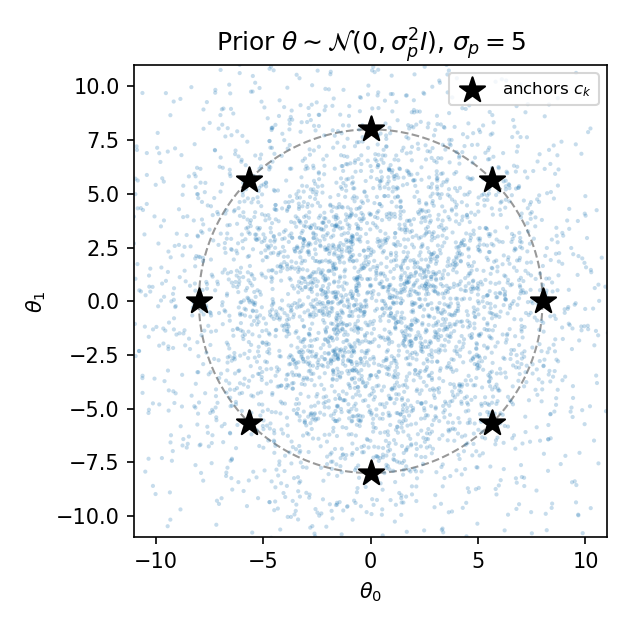
\includegraphics[width=0.52\textwidth]{figs/prior.png}
  \caption{Prior $\theta\sim\mathcal{N}(0,\sigma_p^2 I)$ (blue), a single broad isotropic
  Gaussian. Black stars mark the eight anchors $c_k$ on the dashed circle of radius
  $\rho=8$.}
\end{figure}

\begin{figure}[h]
  \centering
  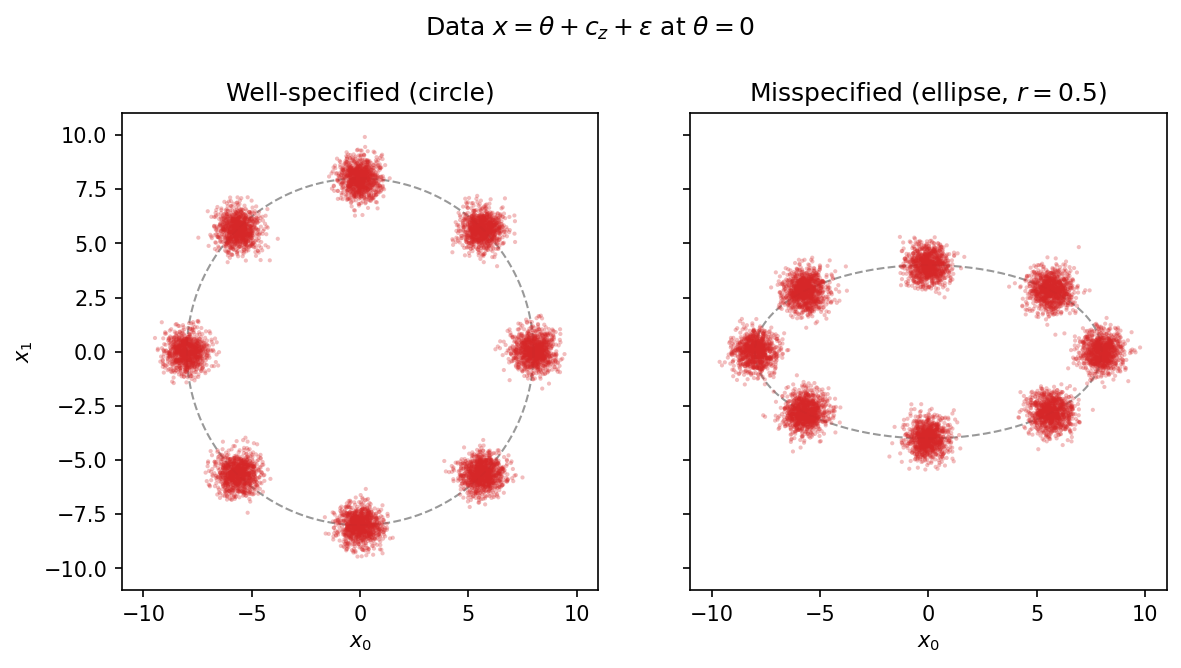
\includegraphics[width=0.95\textwidth]{figs/data.png}
  \caption{Conditional data distribution $x \mid \theta=0$. \emph{Left:} well-specified
  model --- the eight noisy clusters sit on the dashed circle. \emph{Right:} misspecified
  model with \texttt{axis\_ratio}$=0.5$ --- the same clusters now sit on an ellipse.}
\end{figure}

\begin{figure}[h]
  \centering
  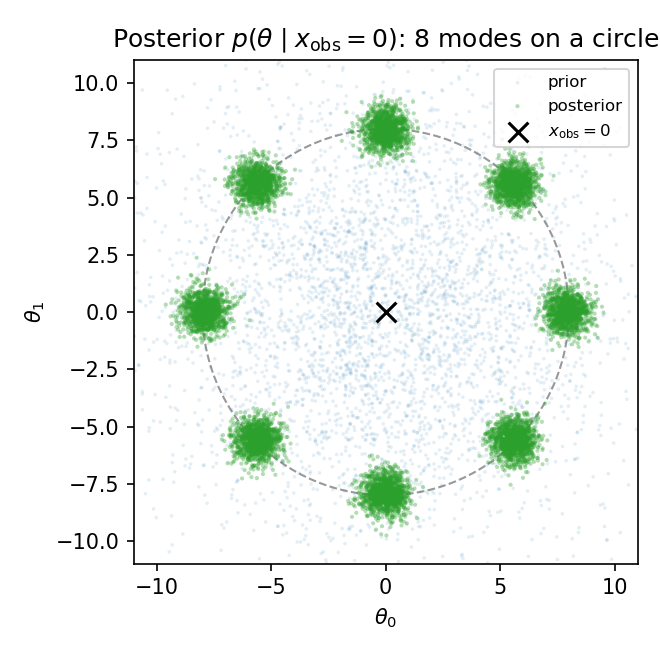
\includegraphics[width=0.55\textwidth]{figs/posterior.png}
  \caption{Closed-form posterior $p(\theta\mid x_{\mathrm{obs}}{=}0)$ (green): eight
  equal-weight Gaussian modes on a circle, sharply concentrated relative to the prior
  (faint blue). The observation $x_{\mathrm{obs}}=0$ is the symmetric point (black cross).}
\end{figure}

\section{Posteriors for other observations $x$}

The point $x=0$ is special only because it is equidistant from all anchors. For a general
observation the posterior is still the eight-component mixture \eqref{eq:post}, but two
things change. From $\mu_k = \frac{\tau^2}{\sigma^2}(x - c_k)$, the eight modes still lie on
a circle of radius $\approx\rho$, now \emph{re-centered} at $\approx x$. From
$w_k \propto \exp\!\big(-\lVert x - c_k\rVert^2 / 2(\sigma_p^2+\sigma^2)\big)$, the weights
\emph{tilt} toward the modes whose anchor $c_k$ is nearest to $x$. Here the denominator
$\sigma_p^2+\sigma^2\approx25.25$ is moderate, so the tilt is pronounced: e.g.\ at $x=0$
all $w_k=0.125$, while at $x=(6,6)$ the weights range over $[0.002,\,0.48]$ --- a couple
of modes dominate and the far ones all but vanish. Figure~\ref{fig:otherx} illustrates
this for four observations.

\begin{figure}[h]
  \centering
  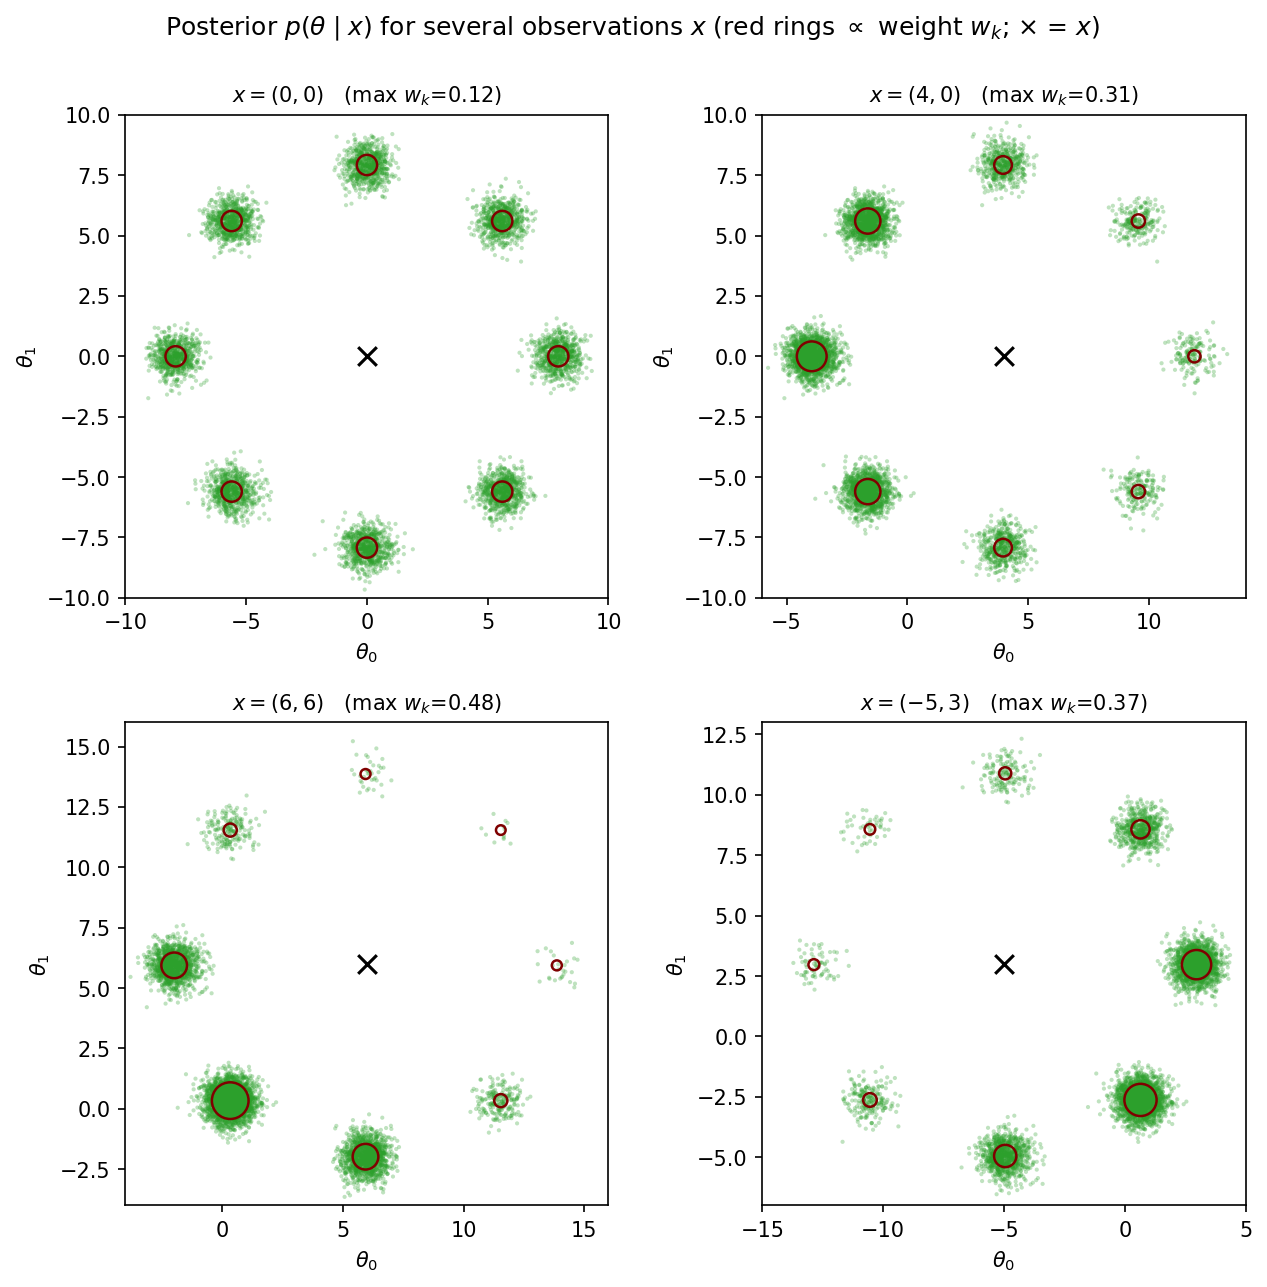
\includegraphics[width=0.82\textwidth]{figs/posterior_other_x.png}
  \caption{Posterior $p(\theta\mid x)$ (green samples) for four observations $x$ (black
  $\times$). Red rings mark the closed-form mode means $\mu_k$, with area proportional to
  the mixture weight $w_k$. As $x$ moves, the ring of eight modes re-centers near $x$ and
  the weights tilt toward the modes nearest $x$ (the per-panel maximum $w_k$ is shown in
  each title).}
  \label{fig:otherx}
\end{figure}

\end{document}
